\par The two dimensional implementation of the electrical, photonic, or metatronic analog approximate \acrshort{pde} solving algorithm needs to operate as close to $O(1)$ constant time as possible in order to provide a useful analog advantage. Figure \ref{fig:2_01_computational_time_complexity} indicates the number of sources and samples needed as well as the limits of mesh dimensions in order to stay in constant time, and therefore potentially be incorporated as an analog accelerator into, as an example, the commonly used digital parallelized multi-grid method operating at a logarithmic $\Theta(\log x)$, polylogarithmic $\Theta(\log^2 x)$, or fractional Power $\Theta(\sqrt{x})$ time complexity, depending on course fine gird traversal for a grid with $x$ grid points. 

\begin{figure}[ht]
\centering\fbox{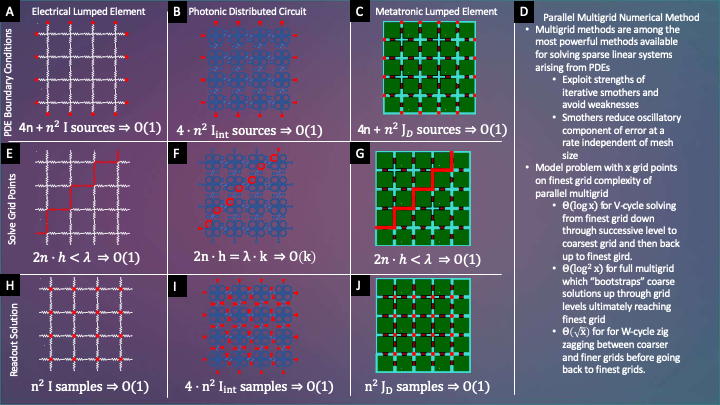
\includegraphics[height=3in,width=5.5in]{figures/figures2/01_computational_time_complexity.png}}
\caption{Computation time complexity of a single PDE analog grid solution iteration in the three analog physics technologies could be incorporated into a \textbf{(D)} parallelized  multi grid method using finite difference method operating at logarithmic time, polylogarithmic time, or fractional power time depending on the course fine grid traversal utilized. For one of the analog system to remain in the constant time domain certain hardware requirements must be met. If we assume that $n$ is the number of nodes in a one dimension side of an grid and $h$ is the length of an edge between nodes in the grid, we can see that the number of \textbf{(A)} current, \textbf{(B)} optical intensity, and \textbf{(C)} displacement current density hardware source locations are needed to set boundary conditions, shown on the top row, and we can see the needed number of \textbf{(H)} current, \textbf{(I)} optical intensity, and \textbf{(J)} displacement current density sample locations are  required to read out a PDE analog solution. With all of these sources and samples operating in parallel. The grid length scales for the \textbf{(E)} electrical \textbf{(G)} metatronic execution step remain within one operation wavelength for both technologies, and thus remain in constant time, where as the \textbf{(F)} photonic grid length scale exceeds its operational wavelength, and thus requires $k$ iterations to traverse the diameter of the grid}
\label{fig:2_01_computational_time_complexity}
\end{figure}







